
%\documentclass[preprint,authoryear,12pt]{elsarticle}
\documentclass[times, 12pt,a4paper]{article}
\usepackage{graphicx,amssymb,amsthm,stmaryrd}%,booktabs}
\usepackage{times}
\usepackage{amsmath,url,algorithm,algorithmic,mathrsfs,makeidx}
\usepackage{graphicx}
\usepackage{epstopdf}
\usepackage{epsfig}
\usepackage{latex8}

%journal{Journal of Knowledge-Based Systems}



\begin{document}
%\begin{frontmatter}

\newtheorem{definition}{Definition}
\newtheorem{proposition}{Proposition}
\newtheorem{example}{Example}
\newtheorem{lemma}{Lemma}
\newtheorem{theorem}{Theorem}
\newtheorem{corollary} {Corollary}
\title{\underline{Response Letter}\\\vspace{0.5cm}Efficient Community Formation for Web Services}
\author{Ehsan Khosrowshahi Asl\\
e\_khosr@encs.concordia.ca\\
\and
Hadi Otrok\\
hadi.otrok@kustar.ac.ae \\
\and
Jamal Bentahar\\
bentahar@ciise.concordia.ca \\
\and
Rabeb Mizouni\\
rabeb.mizouni@kustar.ac.ae \\
}


\maketitle


First, we would like to thank and express our appreciation to the
reviewers for taking the time to carefully review our manuscript,
and for their insightful, valuable, and very useful comments. We
would like to thank the editor as well for his valuable comments
and suggestions for improvements. We carefully considered the
comments and implemented all of them in the revised version. In
this letter, we will explain, point by point, how the issues
raised in the reviews are addressed and answered.

%\newpage

%%%%%%%%%%%%%%%%%%%%%%%%% REVIEWER 1 %%%%%%%%%%%%%%%%%%%%%%%%%
\begin{center}
  \textbf{Reviewer 1}
\end{center}

\vspace{0.4cm}\textbf{\underline{1. Reviewer}:}
You should relate V(S) to PO(C) in equations 5 and 6.

\vspace{0.2cm}\textbf{\underline{Answer 1}:
The connection between V(S) to PO(C) has been already defined when describing the algorithm of our scenario in section 4.1. To clarify it more, we modified the section and we added the connection at the end of the paragraph.
}
% RABEB: I do not get what you mean by however we had .... I beleive taht you need to reformulate your answer by saying that : The connection between V(S) to PO(C) has been already defined when describing the algorithm of our scenario in section 4.1. To clarify it more, we modified the section and we added the connection at the end of the paragraph.


%\vspace{0.4cm}\textbf{\underline{2. Reviewer}:}
%please add some definitions such as the one for Grand coalition
%to make the paper self-contained.

%\vspace{0.2cm}\textbf{\underline{Answer 2}:
%Great suggestion, we did add more definitions for second scenario too.
% RABEB : Cite the definitions you added we did add the definitions of Grand coalition, .....
%}


\vspace{0.4cm}\textbf{\underline{3. Reviewer}:}
Why you didn't leverage the foundations of repeated games instead of
coalitional games? Is there any strong reason?.

\vspace{0.2cm}\textbf{\underline{Answer 3}:
Communities can be seen as cooperative groups where members of the same community cooperate  to achieve a better outcome. In this context, cooperative game theory methods provide us with great decision mechanisms for forming groups and coalitions which would benefit the agents involved altogether. In repeated games, there should be a repeatable game between agents one to one. The  decision cannot be optimal for all the agents involved. We believe repeated game is more appropriate in cases where there is a lot of competing one-to-one interactions between agents  happening and not in coalitions.
 %and actually we are working on repeated games and specifically repeated game with learning techniques such as q-learning to help distribute the ``task distribution job'' among all the web services where web services are having different confidence states, and based on their action history and state they are in, web services can directly opt for getting and performing tasks alone or cooperating which other agents.
}
% RABEB: I do not see the need for the last sentence starting from and actually we are as you are opening the door for questioning our decision  ...



\vspace{0.4cm}\textbf{\underline{4. Reviewer}:}
What do you mean by "the algorithm gets interrupted": is it based on
a logical condition? if yes, what is it?

\vspace{0.2cm}\textbf{\underline{Answer 4}:
It means if there is time constraint, the algorithm can get interrupted any time, and yet has depth(n-1) results. Each depth will have $O(n^2)$ cases to check, so for example if in 5 second it reaches depth 10, and we interrupt the algorithm since we cannot wait any longer,  we at least have checked for all subsets of depth 9}


\vspace{0.4cm}\textbf{\underline{5. Reviewer}:}
Please provide equations using lambda and epsilon and relate them
to your model that uses Rc.

\vspace{0.2cm}\textbf{\underline{Answer 5}:
We added the new stability($Core$ condition) in case of having taxation (Page 10, Equation 8).
}
%RABEB: can you please specify where you have added this

\vspace{0.4cm}\textbf{\underline{5. Reviewer}:}
For the epsilon core method: the value of epsilon should be
varied to verify its impact in the experiments section.

\vspace{0.2cm}\textbf{\underline{Answer 5}:
Yes, the value of epsilon should vary to verify its impact and that is exactly what we are doing. We changed  the explanation to make this fact  more clear.}

\vspace{0.4cm}\textbf{\underline{6. Reviewer}:}
The experiments are missing a comparison with [18] is missing.

\vspace{0.2cm}\textbf{\underline{Answer 6}:
The experiment which was illustrated in figure[9] presents a comparison of our work with [18]. We have called their method ``High Availability Coalition Method''.
 }

\vspace{0.4cm}\textbf{\underline{7. Reviewer}:}
Scalability evaluation is missing: what is the impact of increasing the number of services/communities on the system efficiency?.

\vspace{0.2cm}\textbf{\underline{Answer 7}:
Actually we tried scalability tests, however they did not provide us any special results, since
as mentioned in the paper, our algorithms run in $O(n)$ and $O(n^2)$ time as number of web services within a community (n) grows, so basically our algorithms run in instant time. Also with the real web service data provided in http://www.uoguelph.ca/\textasciitilde{}qmahmoud/qws/, the largest communities used in our experiments did not grow larger than 60 web services. Increasing number of tasks also will not effect us, since communities would only accept tasks at rate $R_C$. However in cases where $R_C$ is set very large, communities can grow larger, and bottleneck of huge number of task processing on a single server, is out of scope of this paper.
large. 
}
%RABEB: it is not clear what you would like to say in the last sentence.


%%%%%%%%%%%%%%%%%%%%%%%%% REVIEWER 2 %%%%%%%%%%%%%%%%%%%%%%%%%
\vspace{2cm}

\newpage

\begin{center}
  \textbf{Reviewer 2}
\end{center}

\vspace{0.4cm}\textbf{\underline{1. Reviewer}:}  Though there�s a referral to [8] it�d be helpful to explain more the concept of �Community coordinators� web services, somewhere in the early parts of the paper. How�s it different from other (common) web services in a given community.

``community master'' and ``community coordinator'' � are these different?


\vspace{0.2cm}\textbf{\underline{Answer 1}: We changed the way  we described our architecture. We dropped the concept of community master web service and we defined  community coordinator.}

\vspace{0.4cm} \textbf{\underline{2. Reviewer}}: p.10 ``our community receives 130 tasks from users'' what are the types of tasks. Are these simulated or real functions that need to performed by web services?

\vspace{0.2cm}\textbf{\underline{Answer 2}: The tasks are randomly generated, and since communities are composed of web services performing the same type of operations, the tasks have the same functional requirement and are of the same type. In our implementation, we let communities perform tasks, and based on community task queue delay and also the assigned web service quality metric such as reliability, throughput, latency and other metrics, these tasks will be performed with different qualities which in excremental results and analysis section we have evaluated and illustrated the results as average QoS of tasks performed
%Rabeb: can you please add where we have presented these results
}


%%%%%%%%%%%%%%%%%%%%%%%%% REVIEWER 3 %%%%%%%%%%%%%%%%%%%%%%%%%
\vspace{2cm}

\newpage

\begin{center}
  \textbf{Reviewer 3}
\end{center}

\vspace{0.4cm}\textbf{\underline{1. Reviewer}:}  It is not convincing that the formation of service community can be modeled as a cooperative gaming problem. First, the concept of service community used in this paper is different from the ones used in the existing work, such as in the referred papers. The general idea of service community is a homogeneous service group that conceptually include services providing similar functionality. Services in the same community are independent and autonomous. There is no central control mechanism for the community. On the other hand, the concept of service community of this paper is a group of services which are monitored and managed by a community manager. It is not clear how realistic or practical such a community is and what the real world examples are.


\vspace{0.2cm}\textbf{\underline{Answer 1}: Most of the existing work such as [Liu 2012][18] (Coordinators), [Lim 2012][16] (Master Web Services], [Benatallah 2003][9] (Service Containers), [Maamar 2008][14], [Maamar 2009][8] (Master Web service), [Zeng 2003][11] (Service selection and task delegation), [Medjahed 2005][13] (Community Providers), [Limam 2010]\footnote{Managing Web Services Communities: A Cache for Queries Optimisation, International Journal on Web Service Computing, Vol.1, No.1, pp 2230-7702, 2010} (Centralized access in their community definition), have clearly stated that communities of web services need a centralized manager for the purposes of developing, coordinating and managing the community and in some of the works, being the access point of the community and having the task of delegating tasks.  We have added a web service community related work section in section I to highlight this point.
}



\vspace{0.4cm}\textbf{\underline{2. Reviewer}:}  The problem is modeled in a way so that the cooperative game theory can be applied, but not in a way that is consistent with the real world scenarios. The service parameters, such as its request rate and throughout rate are not in line with the general characteristics of web services, such as input and output parameters. It is not clear how the proposed service parameters are obtained and why they are important to determine a service's membership to a community, considering that they depend on not only the service's capacity, but also the amount and frequency of user requests, which can be random.


\vspace{0.2cm}\textbf{\underline{Answer 2}: For web services quality metrics, we have used a real world data set provided at: http://www.uoguelph.ca/\textasciitilde{}qmahmoud/qws/. Having a request rate for communities cannot be unrealistic, here is a real world example: Kooshiar Azimian. CEO of concertboom.com has provided me with their access and request rates of the web services they use\ref{cblog}. Their website provides ticketing information for events happening close to user's location. They use Ticketnetwork.com web services\footnote{Affiliate program link: http://www.ticketnetwork.com/affiliates/agreement.aspx} \footnote{Web Service API documentation: http://www.getacoder.com/data/projects/77613/TicketNetwork\%20Web\%20Services\%20(W2)-.doc}, \footnote{We were asked not to enclose these data publicly, that's why we could not add them to the paper} and have implemented their back-end code in Java. They currently almost have 340,000 daily page views, so they call the ticketnetwork web service almost 4 times per second to get the seating chart and tickets available for the events. During a day, the pick time happens at around 20:00 UTC time, which has almost 10\% more request rates than around the lower pick which is around 7:00 AM UTC time. Therefore basically ticketnetwork, knows concertboom.com as a user has a request rate of 340,000 requests per day or almost 3.95 requests per second and they can adjust and change these thresholds, and adjust the internal service providers and resources they have to provide these rate of services.
}

\begin{figure}
\begin{center}
%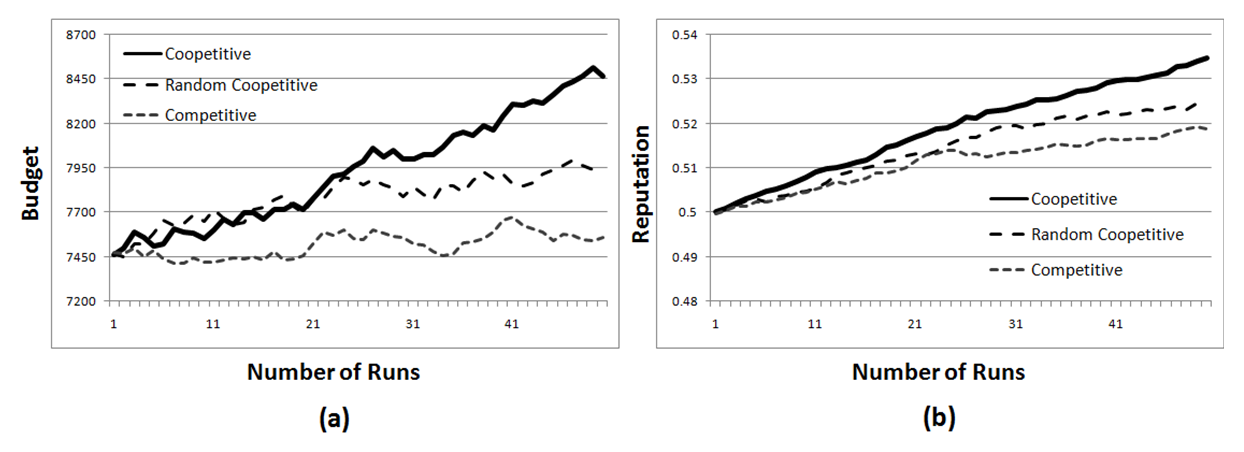
\includegraphics[scale=0.6]{graph1Final+.eps}
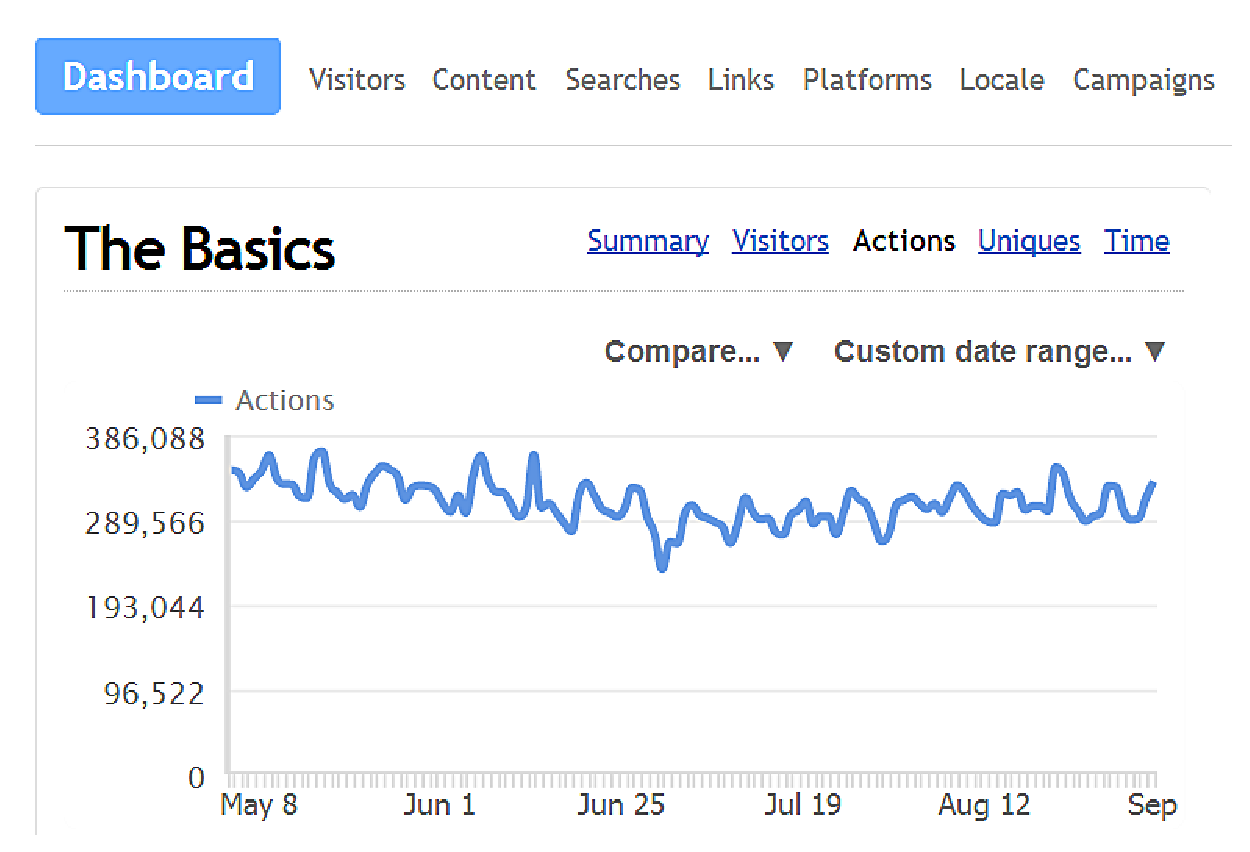
\includegraphics[width=10cm]{cb.eps}\label{cblog}
\caption{Number of ticket pageviews of concertboom.com during May 5th, until Sep 9th, 2013}
\end{center}
\end{figure}

\vspace{0.4cm}\textbf{\underline{3. Reviewer}:}  The paper conducted a simulation instead of an experimental study using real world web services. This also suggests the difficulties of finding real world examples and application for the proposed idea.


\vspace{0.2cm}\textbf{\underline{Answer 3}:
%Our focus is on non-functional properties of web services and is extendable to any type of web service communities providing any type of service, which there is high demand, request load and competition for that service type such as mapping, weather, ticketing, and local places information.
 As mentioned in previous answer we used a real data set of web services (http://www.uoguelph.ca/\textasciitilde{}qmahmoud/qws/) for our implementations. We also added a functional SOAP (XML) messaging system to our implementation, however this as expected did not affect our simulation results, since our concern, as most of the related work, is on non-functional properties of web services. We could deploy web services using JAX-WS in Java and deploy on different servers, however those web services would not reflect the quality of service parameters of real web services under load in real world, however those data set provides of with QoS values of real functioning web services online.
 Similar works on web service community or composition such as
[Yu 2013]\footnote{Q. Yu and A. Bouguettaya, Efficient Service Skyline Computation for Composite Service Selection, IEEE Transactions on Knowledge and Data Engineering (TKDE), vo. 25, no. 4, pp. 776-789, 2013},
[Limam 2010]\footnote{Managing Web Services Communities: A Cache for Queries Optimisation, International Journal on Web Service Computing, Vol.1, No.1, pp 2230-7702, 2010}, and
[Liu 2012]\footnote{A. Liu, Q. Li, L. Huang, S. Ying, and M. Xiao,Coalitional game for community-based autonomous web services cooperation, IEEE Transactions on Services Computing, vol. 99, no. PrePrints, 2012.} the contribution which we have extended their work,
have evaluated their results using simulations.
}




\vspace{0.4cm}

\vspace{1cm}


Finally, we hope that we have answered all the questions raised by
the reviewers, which will make the paper accepted for publication
in IEEE Transactions on Services Computing (TSC).





{
%\bibliographystyle{plain}
%\bibliography{omar}
}
\end{document}
